% ICS paper, high IPC realization
%
%\documentclass[10pt,twocolumn,dvips]{article}
\documentclass[10pt,dvips]{article}
\usepackage[english]{babel}
\usepackage{epsfig}
\usepackage{fancyheadings}
%\usepackage[T1]{fontenc}
%\usepackage[latin1]{inputenc}
%\usepackage{twocolumn}
\usepackage{verbatim,moreverb,doublespace}
\usepackage{rotate,lscape,dcolumn,array,rotating,latexsym}
%\usepackage{overcite}
\usepackage{afterpage,float}
%\usepackage{chbibcor}
%\usepackage{multicol}
%
%
%\renewcommand{\baselinestretch}{1.67}
%\renewcommand{\baselinestretch}{1.55}
\renewcommand{\baselinestretch}{1.00}
%
%
%\input{epsf}
%
%\textwidth 175mm
\textwidth 6.6in 
%\textheight 239mm
\textheight 9.0in
%\leftmargin -2.0in
%\textheight 225mm
%\topmargin -15mm
%\topmargin -4.5mm
\topmargin -0.6in
%\oddsidemargin 0mm
\oddsidemargin 0.0in
%\evensidemargin 0mm
%
%\pagestyle{empty}
%
% 
\newtheorem{theorem}{Theorem}
\newtheorem{lemma}[theorem]{Lemma}
\newcounter{corollary}
\newtheorem{corollary}{Corollary}

\newenvironment{proof}{
\begin{list}{}{
\setlength{\parsep}{0in}
\setlength{\rightmargin}{0.0in}
\setlength{\leftmargin}{0.3 in} 
\setlength{\labelwidth}{0.2 in}
\setlength{\labelsep}{0.1 in} 
\setlength{\listparindent}{1pc}
} 

\item [{\bf Proof}]
}


%\renewcommand{\thefootnote}{\Alph{footnote}}
\renewcommand{\arraystretch}{1.05}

\setlength{\extrarowheight}{1pt}


\newcommand{\helcaption}[1]{\caption{#1}}
%\newcommand{\helcaption}[1]{\caption{\textsf{#1}}}
%\renewcommand{\thefigure}{\textsf{Figure \arabic{figure}: }}
%\renewcommand\figurename{\textsf{Figure}}
%\renewcommand{\thefigure}{\textsf{\arabic{figure}}}
\renewcommand{\thefootnote}{}


\begin{document}
\begin{spacing}{1}

\noindent
{\large University of Rhode Island\\
Dept.\ of Electrical and Computer Engineering\\
Kelley Hall\\
4 East Alumni Ave.\\
Kingston, RI 02881-0805, USA\\}
\vspace{0.15in}

\noindent
{\Large Technical Report No.\ 032002-0101}
\vspace{0.30in}


\begin{center}
{\LARGE \bf 
Realizing High IPC Through a Scalable Memory-Latency Tolerant\\
Multipath Microarchitecture\\
\vspace{0.15in}
}
%
A. Khalafi, D.A Morano,  D.R. Kaeli\\
\{akhalafi, dmorano, kaeli\}@ece.neu.edu\\
Department of Electrical and Computer Engineering\\
Northeastern University\\
and \\
A.K. Uht \\
uht@ele.uri.edu \\
Department of Electrical and Computer Engineering\\
University of Rhode Island\\ 
%
\vspace{0.10in}
%
2nd April 2002\\
%
\vspace{0.11in}
%
{\it This work has been submitted for publication.}\\
%
\vspace{0.30in}
%
\end{center}
\end{spacing}



%\begin{comment}

\footnotetext{This work was partially 
supported by the National Science Foundation through
grants MIP-9708183 and EIA-9729839; by the URI Office of the Provost; 
and by the Spanish Ministry of Education.
Patents applied for. A version of this work has been submitted for
publication. Copyright �� 2001, the 
authors.}

%\end{comment}

\vspace{-0.35in}

%
%
%
%
%\thispagestyle{empty}
%


%
\begin{abstract}
This paper explores a microarchitecture that achieves high execution
performance on conventional single-threaded program codes without
compiler assistance.  Microarchitectures that can have several hundreds
of instructions simultaneously in execution can provide a means to extract
larger amounts of instruction level parallelism, even from programs
that are very sequential in nature.  However, several problems are
associated with such microarchitectures, including scalability
issued related to control flow and memory latency.

We present a basic overview of our microarchitecture and discuss how it
addresses scalability as we attempt to execute many instructions 
in parallel.
We also show how we use
multipath execution to limit the impact of 
conditional branch mispredictions.  We provide simulation results for several
geometries of our microarchitecture that illustrate how high IPC
can be realized from integer programs.  We also explore algorithms
that dynamically reassign speculative paths, reallocating hardware 
resources to higher priority paths. 
Finally, we present data that shows the
tolerance of the microarchitecture to
high memory latency.
\end{abstract}
%
%
\section{Introduction}
%
A number of studies into the limits of instruction level 
parallelism (ILP) have
been promising in that they have shown that there is 
a significant amount of parallelism within
typical sequentially oriented single-threaded programs
(e.g., SpecInt-2000).  
The work of researchers like
Lam and Wilson ~\cite{Lam92},
Uht and Sindagi ~\cite{Uht95},
Gonzalez and Gonzalez ~\cite{Gon97}
have shown that there exists a great amount of instruction level
parallelism (ILP) that is not being exploited by any existing
computer designs.
Unfortunately, most of the fine-grained instruction level
parallelism inherent in integer sequential programs
spans several basic blocks.  
Data and control independent instructions, that may exist
far ahead in the program instruction stream, need to be
speculatively executed to exploit all possible inherent
ILP.
A large number of instructions need to be fetched
each cycle and executed concurrently in order to achieve this.
We need to find the available program ILP at runtime; we need to 
provide sufficient hardware to find, schedule,
and otherwise manage the out-of-order speculative execution of
control and data independent instructions.

The relatively small
instruction fetch windows present on existing processor designs cannot span
the program instruction space necessary to effectively exploit the
available instruction-level parallelism.  
A microarchitecture with a large instruction fetch window and
execution window offers the possibility to both expose (fetch) and
exploit (execute) the available ILP.
For those computer applications that demand the
highest IPC possible on integer codes, a microarchitecture
that is able to execute possibly
several hundreds of instructions speculatively is needed in order to 
maximize execution performance.  

A fundamental challenge 
is how to find program parallelism and then allow execution to occur
speculatively and out of order over a very large number of instructions.
Of course, the microarchitecture has to also provide a means
to maintain the architectural program order that
is required for proper program execution.
It is also usually very desirable to support legacy instruction
set architectures (ISAs) when pursuing high IPC. 
For this reason, we want to explore a
microarchitecture that does not impact the ISA.

We present a novel microarchitecture in this paper that can
be applied to any existing ISA.  Our microarchitecture
is targeted at obtaining
substantial program speedups on integer codes.
The microarchitecture can speculatively execute hundreds
of instructions ahead in the program instruction stream and
thus expose large amounts of inherent ILP.
We use multipath execution to cover latencies associated
with branch mispredictions.
We also take advantage of control
and data independent instructions through our use of
execution-time predication.
Finally, the microarchitecture is also substantially insensitive
to memory component latencies even though it requires higher
memory bandwidth than more conventional machines.

The rest of this paper is organized as follows.
Section 2 presents related work on
high-IPC machines and on multipath execution.
Section 3 presents our proposed microarchitecture.
Section 4 presents simulation results for a range of
machine configurations, and shows the potential
impact of multipath execution when applied.
We also discuss how our microarchitecture reduces
our dependence on the memory system by providing a large
amount of local caching on our datapath. 
Finally, we summarize and conclude in section 5.
%
\section{Background}
%
There have been several attempts at substantially increasing
program IPC through the exploitation of ILP.
The Multiscalar processor architecture \cite{Soh95}
is another attempt at
realizing substantial IPC speedups over convention superscalar
processors.  However, our approach is quite different than theirs
and their approach relies on compiler participation where we do not.
A notable attempt at realizing high IPC was done by
Lipasti and Shen on their Superspeculative
architecture~\cite{Lip97}.  They achieved an IPC of
about 7 with realistic hardware assumptions.
The Ultrascalar machine~\cite{Hen00}
achieves {\em asymptotic} scalability,
but only realizes a small amount of IPC due to its 
conservative execution model.
Nagarajan et al proposed a {\em Grid Architecture} of ALUs
connected by an operand network~\cite{Nag01}.  
This has some similarities to our work.
However, unlike our work, their microarchitecture
relies on the coordinated use of the compiler along with
a new ISA to obtain higher IPCs.

Early work on multipath execution was
dominated by IBM in the
late 1970s and 1980s \cite{Conners79}.
The earliest attempts at multipath
execution started with the ability to prefetch down both
outcomes of a conditional branch.  This became more aggressive
to the point of actually executing down both outcomes of
a conditional branch.  This has
been explored in work such as that by
Wang \cite{Wang90}.  
More aggressive research by Uht and
Sindagi \cite{Uht95} explored the intersection of both
multipath execution and future large-scale microarchitectures
capable of possibly hundreds of instructions being executed simultaneously.
They also addressed the general question of speculatively executing
more than two paths simultaneously.
Work on dual path execution (only two speculative paths) has
been done by Heil and Smith~\cite{Heil96}.
Klauser et al 
explored multipath execution (including more than two
speculative paths)
on the PolyPath microarchitecture ~\cite{Klauser98}.

Exploring multipath execution in the context of
simultaneous multithreading (SMT)
has been done by
Wallace et al \cite{Wallace98}.  
Ahuja et al \cite{Ahuja98} explore some limits for speedups from
multipath execution but their work is still largely restricted to more
conventional (modest sized) microarchitectures.
Our present work explores the use
of multipath execution on a significantly larger scale
than that of Ahuja or most previous work.
%
%
\section{Microarchitecture Description}
%
The microarchitecture is very aggressive in terms of
the amount of speculative execution it performs.
This is realized through a large amount of scalable execution
resources.
Resource scalability
of the microarchitecture is achieved through its distributed nature
along with repeater-like components that limit the maximum bus
spans.
Contention for major centralized structures is avoided.
Conventional centralized resources like a register file,
reorder buffer, and centralized execution units, are eliminated.

The microarchitecture also 
addresses several issues associated with conditional branches.
Spawning alternative speculative paths when encountering conditional
branches is done to avoid branch misprediction penalties.
Exploitation of control
and data independent instructions beyond the join of a 
hammock branch ~\cite{Fer87}
is also capitalized upon where possible.
Choosing which paths in multipath execution should
be given priority for machine resources is also addressed
by the machine.
As shown by Uht and Sindagi ~\cite{Uht95},
equal priority to all simultaneous paths
of a program is not the most efficient use of hardware resources.
The predicted program path is referred to as the \textit{mainline} path.  
We give execution resource priority to this mainline path with respect
to any possible alternative speculative paths.  
Since additional speculative paths have lower priority with
respect to the mainline path, they are referred
to as \textit{disjoint} paths.  
The term \textit{disjoint} refers to that fact that the assignment
of execution resources for that path is likely (and should likely) be
deferred in time
as compared with when execution resources are assigned to the mainline
path.  This sort of strategy for the spawning of alternative speculative
paths results in what is termed \textit{disjoint eager execution} (DEE).
This is in contrast to \textit{singlepath} speculative execution
(widely used at the present)
or \textit{eager execution}.
We therefore refer to disjoint paths as simply \textit{DEE paths}.
These terms are taken from Uht's 1995 work ~\cite{Uht95}.
More detailed information about this microarchitecture
can be found in a technical report by Uht et al~\cite{Uht01}.
%
%
\subsection{High-Level Microarchitecture Components}
%
Figure~\ref{fig:high} provides a high-level view of our microarchitecture.
%
\begin{figure}
%\vspace{0.2 in}
%\setlength{\epsfxsize}{10cm}%7
%\centerline{\epsfbox{window.eps}}
\centering
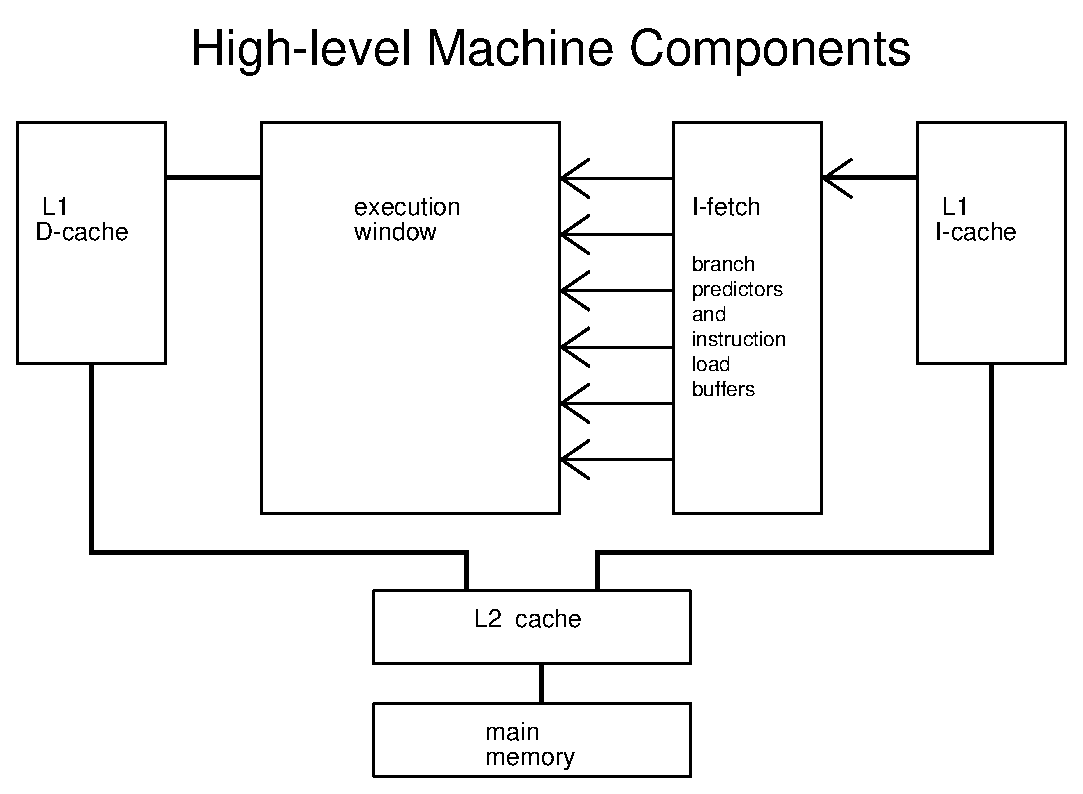
\epsfig{file=high.eps,width=4.0in}
\caption{{\em High-level View of the Distributed Microarchitecture.} 
Shown are the major hardware components of the microarchitecture.
With the exception of the 
execution window block, this is similar to most conventional
microarchitectures}.
\label{fig:high}
\end{figure}
%
Our microarchitecture shares many basic 
similarities to most conventional
machines.
The main memory block,
the L2 cache (unified in the present case), and the L1 instruction 
cache are all rather similar to those in common use.
Except for the fact that the main memory, L2 cache, and L1 data
cache are all address-interleaved, there is nothing further
unique about these components. 
Our L1 data cache is similar to
most conventional data caches except that it also has the ability to
track speculative memory writes.
Our L1 d-cache shares a similar goal with the 
Speculative Versioning Cache \cite{Gop98} 
but is simpler is some respects.
Since we allow speculative memory writes to propagate
out to the L1 data cache, multiple copies
of a speculative write may be present within the L1 data cache
at any time.  They are differentiated from each other
through the use of time-tags.  Time-tags are the basic mechanism
used in the microarchitecture to order all operands, including
memory operands, while they are being used by instructions
currently being executed.  Time-tags are small values that
are associated with operands that serve as both an identifying
tag and as a means to order them with respect to each other.
The Warp Engine~\cite{Cle95}
also used time-tags to manage large amounts of speculative execution,
but our use of them is much simpler than theirs.

The i-fetch unit first fetches instructions from i-cache
along one or more predicted program paths.
Due to our relatively large instruction fetch bandwidth
requirement, we allow for the fetching of multiple i-cache
lines in a single clock.
Instructions are immediately
decoded after being fetched.
All further handling of the instructions is done in their decoded
form.
Decoded instructions are then staged
into an \textit{instruction load buffer}
so that they are available to be loaded 
into the \textit{execution window} when needed.  
The execution window is where
our microarchitecture differs substantially from existing machines.
The transfer of decoded instructions from the instruction load buffer 
to our adaptation of
reservation stations is termed \textit{instruction load}.
This instruction load buffer is organized so that
a large number of instructions can be broadside loaded into the
execution window in a single clock.
The multiple buses going from the i-fetch unit to the
execution window in Figure \ref{fig:high} is meant to
reflect this operation.  
This maximum number of instructions loaded into the
execution window at a time is termed
the \textit{column height} of the machine.  
%
%
\subsection{The Execution Window}
%
Figure \ref{fig:window} shows a more detailed view
of the execution window with its subcomponents.
%
\begin{figure}
%\vspace{0.2 in}
%\setlength{\epsfxsize}{10cm}%7
%\centerline{\epsfbox{window.eps}}
\centering
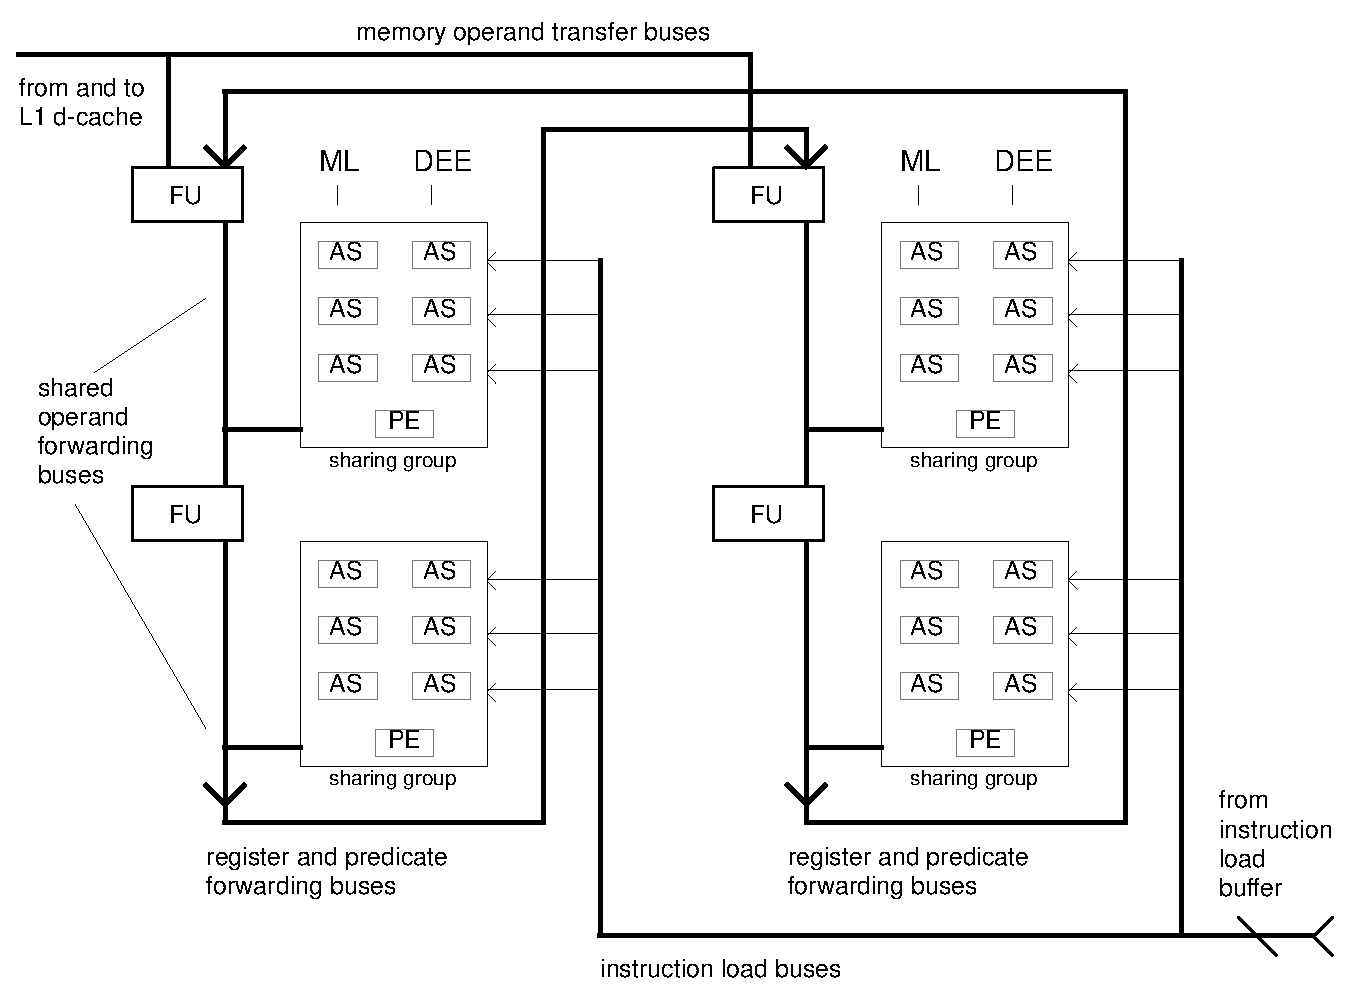
\epsfig{file=window.eps,width=4.5in}
\caption{{\em High-level View of the Distributed Microarchitecture.} 
Shown is a layout of the Active Stations (AS) and Processing Elements (PE)
along with some bus interconnections to implement a large,
distributed microarchitecture.}
\label{fig:window}
\end{figure}
%
We have extended the idea of Tomasulo's reservation
station \cite{Tom67} to provide the basic building block for a distributed
microarchitecture.  Tomasulo's reservation station provided for the
simultaneous execution of different instructions over several
functional units.  
Register results from the functional units were placed on
a common data bus and looped back to provide source register operands 
for instructions waiting in the reservations stations as well as
for updating of the register file.  In our microarchitecture,
an output result is not looped back to the input of the same reservation
station
that provided the result but rather is forwarded to different
stations that are spatially separated, in silicon or circuit board space,
from the first.  
This operation is termed \textit{operand forwarding}.
We call our adaptation of the
reservation station an \textit{active station} (\textit{AS}).
Like a reservation station, an active station can only hold a single
instruction at a time.  After an instruction is loaded into
as AS, it remains there until it can be retired 
(either committed or squashed)  
from the execution window.  
However, instructions can be
re-executed when events indicate that
a re-execution is warranted or required for proper program order
fulfillment.

Rather than lay the ASes out in silicon simply next to
functional units that will execute the instructions loaded to them
(like with the original reservation station idea),
we lay them out in a two dimensional grid whereby sequentially
loaded instructions will go to sequential ASes down a column of
the two dimensional grid of ASes.  
The use of a two dimension
grid simply provides a means to implement the necessary
hardware either in a single silicon IC or through several
suitable ICs laid out in a grid on a circuit board.
The number of ASes in the height dimension of the grid is the
same as the column height of the machine, introduced previously.
The example machine of Figure \ref{fig:high} has a column height of
six (six instruction load buses shown feeding the execution window). 
The column height can also be seen more clearly in 
Figure \ref{fig:window} when the total
number of ASes in a single column of ASes is counted.

Dispersed among the active stations are associated execution
units.  An execution unit is represented in the figure as
a \textit{processing element} (\textit{PE}).  
PEs may consist of an unified all-purpose execution unit capable of
executing any of the possible machine instructions or, more likely,
consist of
several functionally partitioned units individually tailored
for specific classes of instructions (integer ALU, FP, or other),
as is typical of most current machines.
Groups of active stations along with their associated processing
element are termed a \textit{sharing group} (SG).  
They are termed sharing groups because the execution
resources within one of them can be shared among the enclosed ASes.
The example machine of Figure~\ref{fig:window}
consists of two columns of SGs.  
Sharing groups somewhat resemble
the relationship between the register file, reorder buffer,
reservation stations, and function units of most conventional
microarchitectures.  They have a relatively high degree of bus
interconnectivity between them, as conventional microarchitectures do.
The ASes serve the role of both the
reservation station and the reorder buffer of more conventional
machines.
The transfer of a decoded instruction, along with its associated operands,
from an AS to its PE is isolated to within the given SG.
The use of this execution resource sharing arrangement also allows
for reduced interconnections between adjacent SGs.
Basically, only operand results need to flow from one SG
to subsequent ones.

In our present microarchitecture, we always have two 
columns of ASes within a SG.
The first AS column is
reserved for the main-line
path of the program and is
labeled \textit{ML}
in the figure.
The second column of ASes is reserved for the possible
execution of a DEE path and is
labeled \textit{DEE}
in the figure.
In this machine example, each SG contains three rows of ASes
(for a total of six) and a single PE.
Many machine sizes have been explored so far but only a subset
of these sizes is further investigated in this paper.
A particular machine is generally characterized using the tuple: 
%
\begin{itemize}
\item{sharing group rows}
\item{active station rows per sharing group}
\item{sharing group columns}
\item{number of DEE paths allowed}
\end{itemize}   
%
These four characteristic parameters of a given machine
are greatly influential to its performance, as expected,
and is termed the \textit{geometry} 
of the machine.
These four numbers are usually concatenated
so that the geometry of the machine in Figure \ref{fig:window}
would be abbreviated {\tt 2-3-2-2}.

When an entire column
of ASes is free to accept new instructions, generally
an entire column worth of instructions are loaded to the free AS
column from the instruction load buffer, in a single clock.  
Conditional branches are
predicted just before they are entered into the instruction
load buffer (for subsequent load to the ASes).
The prediction of a branch accompanies the decoded instruction
on an instruction load operation.

Also employed within the execution window is a scheme to
dynamically predicate, at execution time, 
all instructions that have been loaded
into active stations.  
This predication scheme essentially provides for each loaded instruction
an \textit{execution predicate}.  These execution predicates
are just a single bit (like with explicit architectural predication)
but are entirely maintained and manipulated within the microarchitecture
itself, not being visible at the ISA level of abstraction.
%
%
\subsection{Operand Forwarding and Machine Scalability}
%
An interconnect fabric is provided to forward result
operands from earlier ASes to 
later ASes, in program order.  
Result operands are one of three possible types: register, memory, and
instruction execution predicates.
The interconnect allows for arbitrary numbers of sharing
groups to be used in a machine while still keeping all bus
spans to a fixed (constant) length.
All of the buses in
Figure \ref{fig:window}, with the exception of the instruction
load buses, form the interconnection fabric.
Several bus arrangements are possible but we only
further explore one such arrangement (that shown in the figure).
In the general case, several buses are used in parallel to make up
a single forwarding span.
This is indicated by the use of the
bold lines for buses in the figure.
More than one
bus in parallel for each bus span is generally required to meet
the bandwidth needs of the machine.

Active bus repeater components are used (and required) to 
allow for constant length bus spans.
A bus repeater component is generally termed a
\textit{forwarding unit} (FU) and is so labeled in the figure.
These forwarding units do more than just repeat operand values from
one span of a bus to the next.
For registers and memory, operands are filtered so that
redundant forwards of the same value (as compared with that last forwarded)
are eliminated.  These can also be termed \textit{silent forwards}.
This filtering provides a means to reduce the overall bandwidth
requirements of the forwarding interconnection fabric.
Each forwarding unit employed in the present work also has a small
amount of storage for memory operands.
This storage serves as a cache for memory operand values.
We term this small cache storage a \textit{L0 data cache}.

For register and predicate operands, values that are generated
by ASes contend for one of the outbound buses
(labeled \textit{shared operand forwarding buses} in the figure) 
to forward the value.
Requests for bus use will be satisfied with any bus clock-slot that may be
available on any of the buses in parallel, belonging to
a given span.  All other ASes on the outbound bus span snoop
operand values forwarded from previous (in program order)
ASes.  In addition, a forwarding unit (the bus repeater) also
snoops the same operands and forwards the operand value to the
next bus span if necessary (if the value was different than the previous
value).  For register and predicate operands, they are also
looped around from the bottom of one column of SGs
to the top of the next column of SGs.  
Operands from the bottom of the
far right column of SGs gets looped around to the
top of the far left column.  
This behavior forms the characteristic ring pattern of operand flow,
inherent in many microarchitectures.  Forming a closed loop
with these buses, and essentially just renaming columns (identifying the
one closest to retirement), is easier than physically transferring
(shifting) the contents of one column to the next when a column
of ASes retires.

For memory operands, we employ a second operand forwarding strategy.
When memory operands are generated by ASes, again the AS contends
for one of the outbound buses 
(labeled \textit{shared operand forwarding buses} in the figure) 
in order to forward the operand value.
However, unlike the register and predicate operand forwarding
strategy, memory operands also travel backwards, in program ordered
time, and get snooped by the forwarding units that are at the top
of each SG column.  This is done so that the operand can
be transfered onto a \textit{memory operand transfer bus}, shown
at the top of Figure \ref{fig:window}.  
These buses are address-interleaved and
provide the connectivity to get memory operands (generally
speculative) over to the L1 data cache.
Values are tentatively stored in the L1 data cache along with 
their associated operand
time-tags until a committed value is determined.
Similarly, operands returning from the L1 data cache to service requests
from ASes, are first put on one of the memory operand transfer buses (based
on the interleave address of the operand).  These operands then get snooped
by all of the forwarding units at the top of each SG
column, after which the operand is forwarded on a shared operand
forwarding bus to reach the requesting ASes.

Persistent register, predicate state and some persistent
memory state is stored in the forwarding units.
Persistent state is not stored indefinitely in any single forwarding
unit but is rather stored in different units as the machine
executes column shift operations (columns of ASes get retired
and committed).  However, this is all quite invisible to the ISA.
This microarchitecture also implements precise exceptions~\cite{Smi88}
similarly to how they
are handled in most speculative machines.  
A speculative exception (whether on the main-line path or a DEE path)
is held pending (not signaled in the ISA)
in the AS that contains the generating
instruction until it would be committed.
No action is needed for pending exceptions in ASes that eventually
get squashed.
When an AS with a pending exception does commit, the machine directs the
architected control flow off to an exception handler through
the defined exception behavior for the given ISA.
This might include saving the precise instruction return
address to either an ISA architected register or memory.
Typically, the exception handler code will save the architected
registers to memory using normal
store instructions of the ISA.
Interrupts can be handled in more flexible ways than exceptions.
One way to handle interrupts is to allow all instructions
currently being executed within the execution window to reach
commitment, then architected program flow can vector off to
a code handler, similarly as the case of instruction exceptions above.
%
%
\subsection{Enforcing Program Order and Dependencies}
%
Program dependencies (control, register, and memory) are 
maintained through the use of time-tags.
Time-tags are associated with all transient operands within the machine.
This has some resemblance to register tags used in more conventional 
microarchitectures but has been more generalized for use in this
distributed microarchitecture.  
Since instructions remain in the ASes that they were loaded into until
they retire, the whole set of ASes
fulfill the role of the reorder buffer or register update unit of more
conventional microarchitectures.
As a column of ASes gets retired, that column becomes available
for the loading of newly decoded instructions.
In addition, a time-tag associated with each column get decremented.
Time-tags associated with operands can be decomposed into row and 
column parts.  The column part of the operand time-tag is
identically the column time-tag, so when a column has its time-tag
decremented, it effectively renames the operands within that column.
The next column in the machine (with the next higher time-tag)
becomes the next column that will get retired.
The operation of decrementing column time-tags 
in the execution window is termed a \textit{column shift}.
The hardware used for the snooping of an input operand of an AS
is shown in Figure \ref{fig:source}.
Basically, a new operand is snarfed when it has the same address and
path identifier as the current AS as well as
a time-tag value that is less than that of the current AS itself
but greater or equal to that of the last snarfed operand.
Simpler snooping hardware is used in forwarding units.
%
\begin{figure}
%\vspace{0.2 in}
%\setlength{\epsfxsize}{14cm}%7
%\centerline{\epsfbox{source.eps}}
\centering
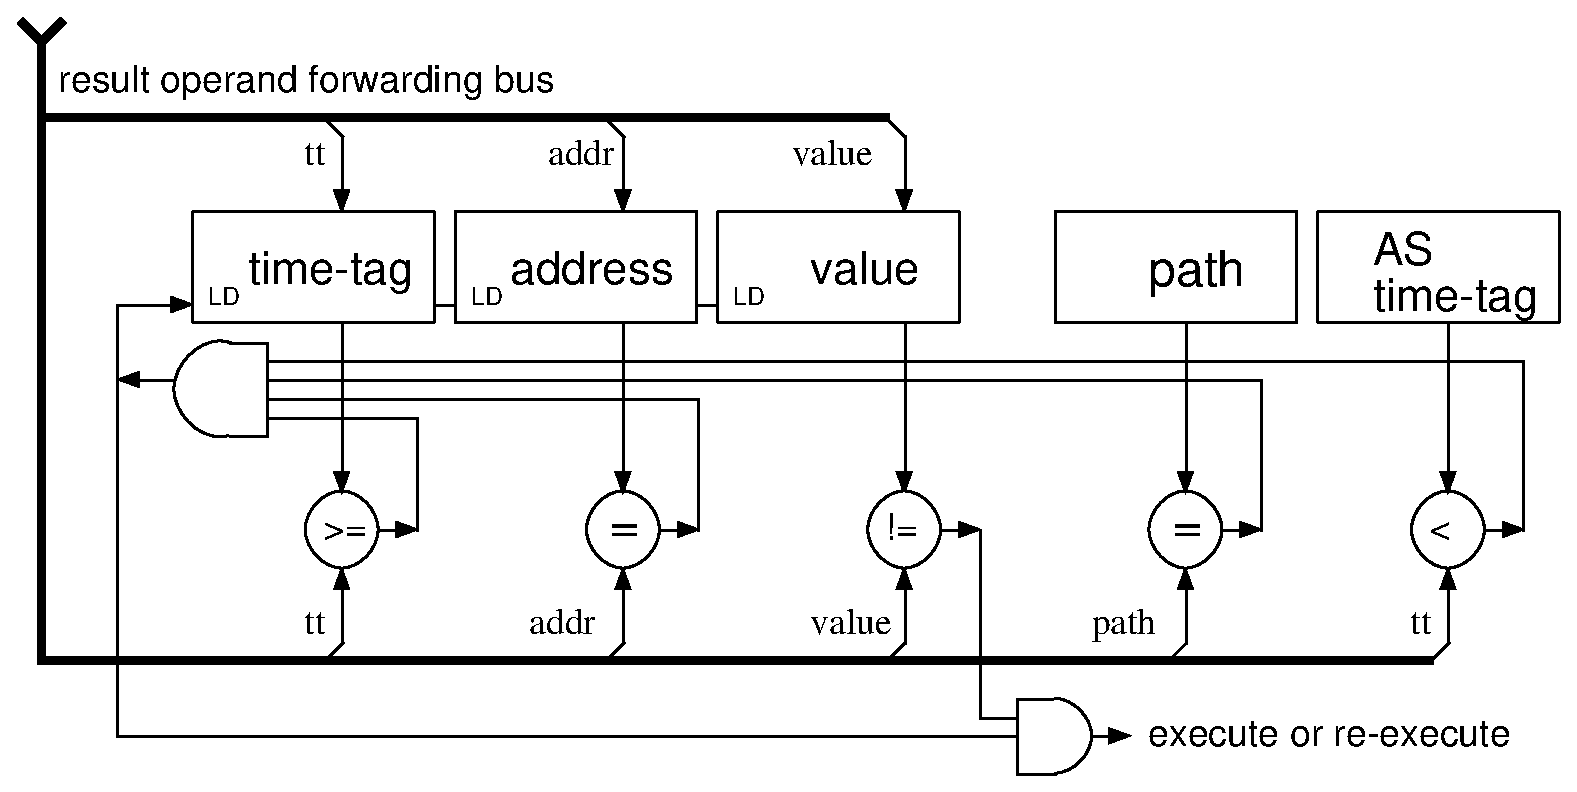
\epsfig{file=source.eps,width=4.0in}
\caption{{\em Operand snoop logic within an AS.}
The logic used for snooping of input operands for ASes is shown.}
\label{fig:source}
\end{figure}
%
A more detailed discussion of the mechanism used for
enforcing program dependencies
can be found in a report by Kaeli et al~\cite{Kaeli01}.
%
%
\subsection{Conditional Branches and Multipath Execution}
%
If a conditional backward branch is predicted taken,
the i-fetch unit
will speculatively follow it and continue loading instructions
into the execution window for the mainline path from the target
of the branch.  
This case allows for the capture of program loops
within the execution window of the machine and can be thought of
as hardware loop unrolling.
For a backward branch that
is predicted not-taken, we continue loading instructions following the
not-taken output path.
If a forward branch has a near target, such
that it can be loaded within the execution window, 
then we load instructions following the
not-taken output path of the branch, whether or not it is the predicted path.
This represents the fetching of instruction in the 
memory or \textit{static} order rather than the program dynamic order and
is very common in the absence of a loop.
The fetching and loading of instructions following the
not-taken output path (static program order) of a conditional
branch is very advantageous for 
capturing hammock styled branch constructs.  
Simple single-sided hammock branches generally have near targets,
they are thus captured within the execution window.

Our mainline path continues along the predicted branch output path
regardless of whether it was the taken or not-taken one.  
We spawn a DEE path
for the opposite output of the branch from
the mainline path case, whatever it is.
For forward branches with a far target,
if the branch is predicted taken, we load instructions following the target
of the branch.  If the branch is predicted not-taken, we continue
loading instructions for the mainline path following the not-taken
outcome of the branch.  In both of these cases, we do not
spawn a DEE path for this branch.

DEE paths are created by loading an available
column of ASes, a free second column of ASes within a SG column, with
the same decoded instructions from the AS column that contained
the conditional branch instruction that gave rise to the DEE path.
However, there are a limited number of AS columns
available at any one time for DEE paths in the machine.
Several strategies for the management of the DEE path AS columns 
are
possible and we present two such strategies in the present work.

One such strategy is very simple and just 
spawns DEE paths for suitable conditional
branches (as explained above) on a first come, first served basis.  
That is, as machine
execution resources that are reserved for DEE paths
become available, those resources are assigned to the next conditional
branch for which a DEE path has not already 
been assigned.  The DEE path is allowed to
remain executing until its originating conditional
branch gets resolved, at which point either it or the corresponding
main-line path is squashed (the other of the two paths commits).

A second strategy that we explore is to monitor
the amount of time that existing DEE paths have been
resident in the execution window, and to squash those paths that
have reached a residency threshold.  Residency time in the
execution window is approximated by the number of column shifts that
have occurred since a DEE path was spawned.  
Again, a column
shift corresponds with the retirement of the AS column with the
lowest valued time-tag.
The rationale is that the longer a DEE path is resident
within the execution window,
the likelihood of the conditional branch that gave rise to it being 
mispredicted becomes less.  
Thus, that DEE path is no longer using the
underlying execution resources as well as maybe some new DEE
path might (remember that the DEE path is used to follow the not predicted
path).
When a DEE path is 
squashed in order to make room for
the spawning of a new DEE path, the associated
execution resources are released and assigned to another conditional
branch.
This is termed the \textit{release} strategy of managing
DEE paths.
%
%
\section{Simulation Results}
%
We first describe our simulation process.
Then results showing IPCs for each of three
modes of execution of the machine is given.
Finally, results showing the sensitivity of our machine
to varying the latencies of several components in the memory hierarchy
is presented.
%
%
\subsection{Methodology}
%
The simulator is a recently built tool that shares some similarity
to SimpleScalar \cite{Austin97} but which was not based on it.
We execute
SpecInt-2000 and SpecInt-95 programs on a simulated machine
that features a MIPS-1 ISA along with the addition of some MIPS-2 and
MIPS-3 ISA instructions.  We are using the standard SGI Irix system
libraries so we needed to also support the execution of some
MIPS-2 and MIPS-3 instructions (present in the libraries).
All programs were compiled on an SGI machine under the
Irix 6.4 OS and using the standard SGI compiler and linker.  
Programs were compiled with
standard optimization ({\tt -O}) for primarily the MIPS-1 ISA ({\tt -o32}).
No changes to the SGI compiler or linker were made to create
the binary benchmark programs.

We chose five benchmark programs to work with,
four from the SpecInt-2000 benchmark suite
and one from the SpecInt-95 program suite.
These programs were chosen to get a range of different memory and looping
behavior, while also presenting challenging conditional control flow
behavior.
The particular programs used along with some statistics 
are given in Table \ref{tab:benches}.
All programs were executed using the SpecInt reference inputs.
All accumulated data was gathered over the simulated execution of
500 million instructions,
after having skipped the first 100 million instructions.
The first 100 million instructions, however, were used to warm up the
various simulator memory caches.
%
\begin{table}
\begin{center}
\caption{Benchmarks Programs Simulated and Some Statistics.}
\label{tab:benches}
\begin{tabular}{|l|c|c|c|c|c|}
\hline 
benchmark&bzip2&parser&go&gzip&gap\\
\hline 
\hline 
br. prediction accuracy&90.5\%&92.6\%&72.1\%&85.4\%&94.5\%\\
\hline 
avg. L1-I hit rate&97.2\%&96.6\%&92.4\%&94.7\%&89.0\%\\
\hline 
avg. L1-D hit rate&98.8\%&99.0\%&98.8\%&99.8\%&99.3\%\\
\hline 
avg. L2 hit rate&90.1\%&86.0\%&96.8\%&73.0\%&88.5\%\\
\hline 
dynamic cond. brs.&12.0\%&11.0\%&12.1\%&13.4\%&6.5\%\\
\hline 
S-S hammock brs.&23.4\%&42.1\%&35.7\%&45.2\%&27.3\%\\
\hline
\end{tabular}
\end{center}
\end{table}
%
The dynamic conditional branches in Table \ref{tab:benches} are
a percent of total dynamic instructions.
The numbers for the Simple Single-sided (S-S)
Hammock branches ~\cite{Fer87,Sank01}
are percentages of total dynamic conditional branches.
%
%
\subsection{IPC Results for Singlepath and Multipath Execution}
%
In this section, we present IPC data for three different 
modes of machine execution, each on five machine geometries.
The execution modes are : no multipath execution (singlepath),
simple multipath execution , and enhanced multipath execution.
The numbers of each of the major machine components, for each of the 
five
simulated geometries, are given in Table \ref{tab:configs}.
Although we have explored a large number of various sized
machines, these particular geometries were chosen in order
to get a range of IPC performance across a number of very
different machine sizes and shapes.
The common machine characteristics used in this section for
obtaining IPC results is given in Table \ref{tab:params}.
The L1, L2, and main memory access latencies do not include
the forwarding unit and forwarding bus delays within the
execution window.
These machine characteristics are fairly representative of
existing typical values for a 2 GHz processor.  
They are similar to, or more conservative
than, a recent Pentium-4 (0.13 um) processor \cite{Lud02}.
%
\begin{table}
\begin{center}
\caption{Machine geometries simulated for each of the benchmark
programs.}
\label{tab:configs}
\begin{tabular}{|c|c|c|c|}
\hline 
SG rows&
ASes per SG&
SG columns&
max D-paths\\
\hline
\hline 
8&4&8&8\\
\hline 
8&8&8&8\\
\hline 
16&8&8&8\\
\hline 
32&2&16&16\\
\hline 
32&4&16&16\\
\hline
\end{tabular}
\end{center}
\end{table}
%
\begin{table}
\begin{center}
\caption{{\em General machine characteristics.}
These machine parameters are used for all simulations as
the default except where one of these parameters may be varied.}
\label{tab:params}
\begin{tabular}{|l|l|}
\hline 
L1 I/D cache access latency&1 clock\\
\hline
L1 I/D cache size&64 KBytes\\
\hline
L1 I/D block size&32 bytes\\
\hline
L1 I/D organization&2-way set associative\\
\hline
L2 cache access latency&10 clocks\\
\hline
L2 cache size&2 MBytes\\
\hline
L2 block size&32 bytes\\
\hline
L2 organization&direct mapped\\
\hline
main memory access latency&100 clocks\\
\hline
memory interleave factor&4\\
\hline
forwarding unit minimum latency (all)&1 clock\\
\hline
forwarding-bus latency (all)&1 clock\\
\hline
number of forwarding buses in parallel&4\\
\hline
branch predictor&PAg\\
\cline{2-2}
 & 1024 PBHT entries\\
\cline{2-2}
 & 4096 GPHT entries\\
\cline{2-2}
 & saturating 2-bit counter\\
\hline
\end{tabular}
\end{center}
\end{table}
%
The IPC results for each of the three modes of machine execution
are presented in Tables \ref{tab:ipc1}, \ref{tab:ipc2}, and \ref{tab:ipc3}.
The geometry labels (4-tuples) 
at the tops of these tables consist of the concatenated 
numbers of
machines components for: SG rows, AS rows per SG, SG columns,
and the number of DEE paths allowed for that execution.

Table \ref{tab:ipc1} gives the IPC results for each of the benchmark
programs, when executing in
singlepath mode.
For singlepath execution, the allowed number of 
DEE paths is zero.

In addition to the individual benchmark IPC results, we also
present the harmonic mean of the IPC across all benchmarks.
Table \ref{tab:ipc2} gives the results using the simple method 
(first-come-first-serve) for
the spawning of DEE paths.
%
\begin{table}
\begin{center}
\caption{IPC results for singlepath execution.}
\label{tab:ipc1}
\begin{tabular}{|c|c|c|c|c|c|}
\hline 
geometry&
8-4-8-0&
8-8-8-0&
16-8-8-0&
32-2-16-0&
32-4-16-0\\
\hline 
\hline
bzip2&3.4&4.2&4.8&4.2&4.7\\
\hline 
parser&2.8&3.3&3.8&3.5&3.9\\
\hline 
go&2.6&3.2&3.6&3.4&3.6\\
\hline 
gzip&3.4&4.4&5.2&4.8&5.3\\
\hline 
gap&4.5&5.6&6.1&6.5&6.3\\
\hline
\hline 
HAR-MEAN&3.2&3.9&4.6&4.2&4.6\\
\hline
\end{tabular}
\end{center}
\end{table}
%
\begin{table}
\begin{center}
\caption{IPC results for multipath execution using the 
simple D-path strategy.}
\label{tab:ipc2}
\begin{tabular}{|c|c|c|c|c|c|}
\hline 
geometry&
8-4-8-8&
8-8-8-8&
16-8-8-8&
32-2-16-16&
32-4-16-16\\
\hline 
\hline 
bzip2&3.9&4.8&5.5&4.9&5.3\\
\hline 
parser&4.0&4.3&5.1&4.6&5.1\\
\hline 
go&4.6&5.6&6.4&5.9&6.3\\
\hline 
gzip&4.7&5.9&6.8&6.2&6.8\\
\hline 
gap&5.6&6.9&7.1&8.3&7.2\\
\hline 
\hline 
HAR-MEAN&4.5&5.4&6.1&5.7&6.1\\
\hline
\end{tabular}
\end{center}
\end{table}
%

Examining the data, we can see that our simple 
(first-come-first-serve)
multipath execution
strategy significantly outperforms singlepath execution.
This was expected as the microarchitecture is able to
capture inside of the execution window 
many of the instructions following both outcomes
of forward conditional branches,
thereby largely hiding any misprediction penalties of those branches.

Next we want to get results for machine simulations using our
more complicated \textit{release} management strategy for DEE paths.
In this enhanced strategy, DEE paths are allowed to
remain within the execution window for a certain number of
columns shifts (described previously).  We first attempt to
determine the best number of column shifts to use as a metric
for path residency.  For this we took one machine geometry and
varied the number of column shifts the machine waits before releasing
a DEE path.
We use the machine geometry of 16-8-8-8 along with the parameters
listed in Table \ref{tab:params}
to investigate
IPC speedups as the number of column shifts waited for is varied.
Figure \ref{fig:release} shows the resulting IPC speedups,
as compared with the simple disjoint path management strategy.
%
\begin{figure}
%\vspace{0.2 in}
%\setlength{\epsfxsize}{14cm}%7
%\centerline{\epsfbox{release.eps}}
\centering
\epsfig{file=release.eps,width=4.0in}
\caption{Machine IPC speedup results for varying 
column shifts.}
\label{fig:release}
\end{figure}
%
For this particular machine geometry, this strategy
performs worse than the simple strategy when the number
of column shifts waited for is 
approximately fewer than four or five.
However, when DEE paths are retained in the
execution window for approximately
six columns shifts,
a performance speedup of about two to five percent is realized
over the simple DEE path strategy.
From these results, we will chose to allow DEE paths
to remain in the execution window for six column shifts
for all five machine geometries explored and all benchmarks.

Table \ref{tab:ipc3} gives the results using the \textit{release} 
method for the spawning of DEE paths.
Again, these allow DEE paths
to stay resident in the execution window through six column shifts
(determined above)
and the remaining parameters of the machine 
are those in table \ref{tab:params}.
%
\begin{table}
\begin{center}
\caption{IPC results for multipath execution using the 
release D-path strategy.}
\label{tab:ipc3}
\begin{tabular}{|c|c|c|c|c|c|}
\hline 
geometry&
8-4-8-8&
8-8-8-8&
16-8-8-8&
32-2-16-16&
32-4-16-16\\
\hline 
\hline
bzip2&4.2&5.0&5.8&5.4&5.7\\
\hline 
parser&4.3&4.6&5.3&5.0&5.4\\
\hline 
go&5.1&5.9&6.7&6.5&6.8\\
\hline 
gzip&5.0&6.3&7.0&6.7&7.2\\
\hline 
gap&6.0&7.5&7.5&8.9&7.9\\
\hline 
\hline 
HAR-MEAN&4.8&5.7&6.4&6.3&6.5\\
\hline
\end{tabular}
\end{center}
\end{table}

%
From these results, 
it is observed that our more complicated DEE \textit{release} strategy
performs better than our simple strategy for all machine
geometries explored here.
This is encouraging and suggests that attention to the
management of the DEE paths is important to getting
higher IPC speedups.
Some other strategies for the management of how and when to
spawn DEE paths have been proposed but they have not yet been
explored.  
This is an area that we intend to explore more
fully in the future.

Our lowest performing machine geometry (8-4-8-8) when executing
in singlepath mode, yielded a harmonic mean IPC of 3.2.
However, the same geometry machine, when executing using the
enhanced DEE path strategy, yielded a harmonic mean IPC of 4.8
(substantially better).  Finally, the largest sized machine geometry
simulated using the enhanced DEE path strategy, yielded a
harmonic mean IPC of 6.5.
%
%
\subsection{Memory Sensitivity Results}
%
In this section we present IPC data corresponding to varying some
parameters associated with the memory subsystem.
We show IPC speedup results for varying the access latencies,
in clocks, for: L1 I-cache,
L1 D-cache,
L2 cache, and
main memory.
All of this data was gathered on a machine geometry 
of 16-8-8-8 with the other parameters (the ones that are
not varied) being those that are listed in Table \ref{tab:params}.
Figure \ref{fig:l1icache} presents the IPC speedups for varying
the L1 I-cache hit latency clocks from one up to eight.
Figure \ref{fig:l1dcache} presents IPC speedup results
as the L1 D-cache hit latency is also varied from one to eight clocks.
For these two figures, the speedups (the ordinate)
range from 0.0 through 1.2.
Figure \ref{fig:l2cache} presents the IPC speedup results
as the L2 cache (unified I/D) hit latency is varied from 
one up to 16 clocks (our design choice was 10 clocks).
Finally Figure \ref{fig:dram} presents the IPC speedup results
as the main memory access hit latency is varied from twenty clocks 
up to 800 clocks.
For the L2 cache and main memory sensitivity graphs, the speedups
(ordinate) range from 0.9 through 1.02.
All IPC speedups in these figures are relative to the 1 clock
access latency cases.  
%
\begin{figure}
%\vspace{0.2 in}
%\setlength{\epsfxsize}{14cm}%7
%\centerline{\epsfbox{l1icache.eps}}
\centering
\epsfig{file=l1icache.eps,width=4.0in}
\caption{Machine IPC speedup results for varying 
L1 I-cache hit delay in clocks.}
\label{fig:l1icache}
\end{figure}
%
\begin{figure}
%\vspace{0.2 in}
%\setlength{\epsfxsize}{14cm}%7
%\centerline{\epsfbox{l1dcache.eps}}
\centering
\epsfig{file=l1dcache.eps,width=4.0in}
\caption{Machine IPC speedup results for varying 
L1 D-cache hit delay in clocks.}
\label{fig:l1dcache}
\end{figure}
%
\begin{figure}
%\vspace{0.2 in}
%\setlength{\epsfxsize}{14cm}%7
%\centerline{\epsfbox{l2cache.eps}}
\centering
\epsfig{file=l2cache.eps,width=4.0in}
\caption{Machine IPC speedup results for varying 
L2 cache hit delay in clocks.}
\label{fig:l2cache}
\end{figure}
%
\begin{figure}
%\vspace{0.2 in}
%\setlength{\epsfxsize}{14cm}%7
%\centerline{\epsfbox{dram.eps}}
\centering
\epsfig{file=dram.eps,width=4.0in}
\caption{Machine IPC speedup results for varying 
main memory access latency in clocks.}
\label{fig:dram}
\end{figure}
%
As can be seen from Figures \ref{fig:l1icache} and \ref{fig:l1dcache},
the machine is slightly more sensitive to L1 D-cache latency
than to L1 I-cache latency.  This is expected due to the
variability in speculative memory accesses that is present for 
data memory accesses,
that is not as prevalent in instruction accesses.
Fortunately, latencies of 1 or 2 clocks
for L1 caches is more likely to scale better with increasing
processor clock rate than memory components further from the processor.

For the L2 cache (ours is currently unified), speedups are
possible when using short clock latencies than the 10 clocks that
we used as our default.
Although L2 latencies are likely to also scale somewhat
with future increasing processor clock rates, they are not likely
to scale as well as L1 is expected to do.
Fortunately our machine already obtains good IPC numbers
for an L2 latency of 10 clocks. 

With respect to main memory, the microarchitecture
is quite insensitive to latencies out to 100 clocks and
only then starts to degrade slightly after that.  
Since 100 clocks
(as we count it -- after our repeater and bus delays)
is probably typical at the present time (assuming a 2 GHz
CPU clock rate and the latest DDR-SDRAMs), our memory system
arrangement is properly hiding most of the long main memory latency as it
should.  
Since our machine is still quite insensitive to
main memory latency out to 800 clocks, we might expect to
operate the current machine up to about 10 GHz with similar performance.
Our insensitivity to main memory latency is due to both the conventional
use of L1 and L2 caches but also to the width of our execution window.
When memory load requests are generated from instructions
soon after they were loaded into
the execution window, the width of the machine (in SG columns) provides
substantial time to allow for those memory load requests to
be satisfied, even when they have to go back to L1, L2, and to
main memory.
%
%
\section{Conclusions}
%
We have presented the overview of a large-scale distributed 
microarchitecture suitable for extracting high ILP from
sequential programs.
This microarchitecture is designed to also implement 
speculative multipath execution.  We presented results
for the machine executing in singlepath mode and two types
of management for alternative speculative paths in multipath mode.
It was shown that multipath execution provides additional IPC
performance over singlepath execution using
both of the heuristics that we explored for
managing the alternative paths.
Further, our enhanced DEE path \textit{release} heuristic provided
an additional average of about five percent better IPC over the
simple DEE path management heuristic for a modest sized machine.
We also showed that our microarchitecture exhibits significant
insensitivity to a wide range of memory system component latencies.
%
\bibliographystyle{latex8}
\bibliography{high}
%
\end{document}
%
%
